\section{Data Modeling}

Since our data looks like a (skewed) bell curve, we model our data using a normal distribution.
Firstly, we use a Box-Cox transformation to reduce the skewness of our data.

Box-Cox transformation with the parameter $\lambda$ is defined as follows:

\[
  \text{Box-Cox}(x_i; \lambda) =
  \begin{cases}
    \frac{1}{\lambda} (x_i ^ \lambda - 1) & \lambda \ne 0 \\
    \ln x_i & \lambda = 0
  \end{cases}
\]

\noindent $\lambda > 1$ increases the data skewness whereas $\lambda < 1$ decreases the skewness.
Box-Cox transformations with various $\lambda$ values are given in \autoref{fig:transforms}.

\begin{figure}[!ht]
  \centering
  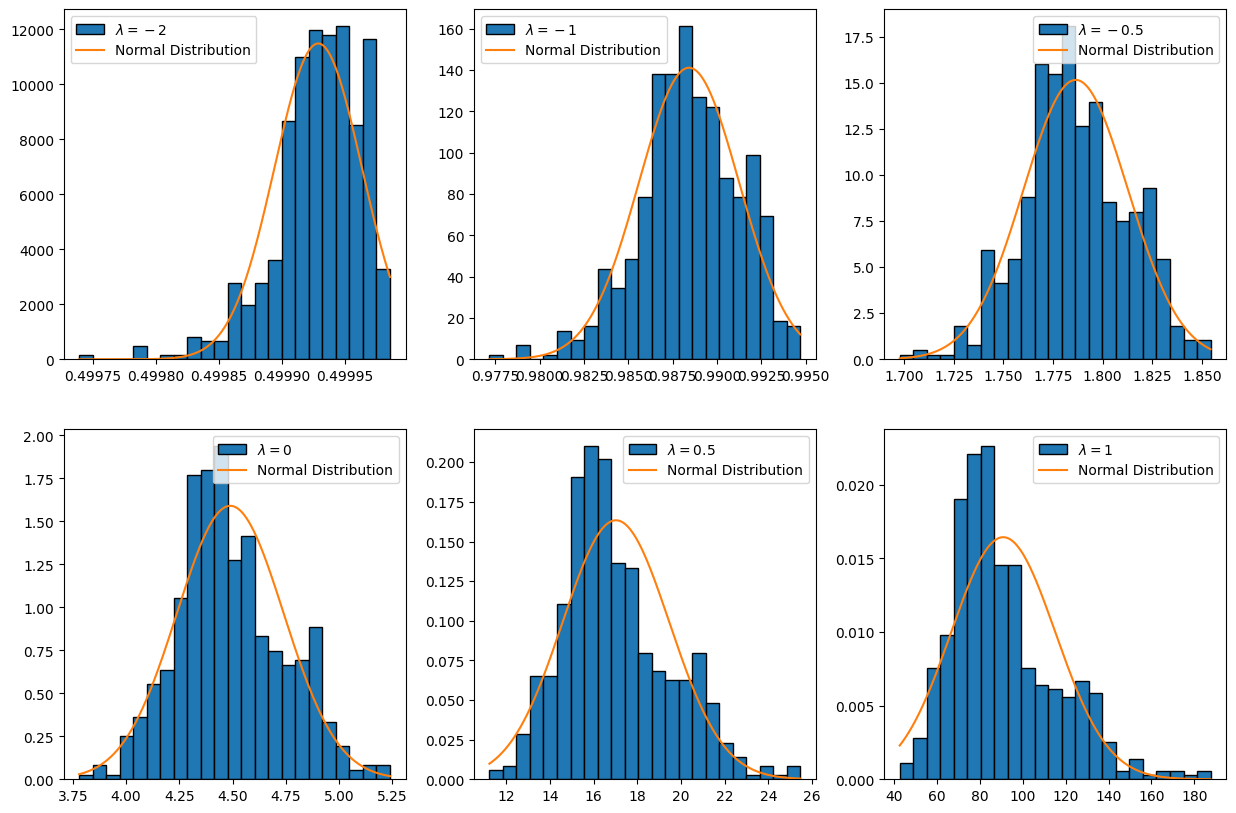
\includegraphics[width=\textwidth]{images/transforms.png}
  \caption{Box-Cox transformations with various $\lambda$ values}
  \label{fig:transforms}
\end{figure}

To visualize how well a transformation fits the normal distribution, we use Q-Q (Quantile-Quantile) plots.
A Q-Q plot is made by plotting the theoretical quantiles against the observed quantiles of the data.
The theoretical quantile corresponsing to $x_{(i)}$ is:

\[ y_i = F^{-1}\left(\frac{i}{n + 1}\right) \qquad i \in \{1, 2, ..., n\} \]

\noindent where $n$ is the number of data points, $x_{(i)}$ is the $i$ th data point in ascending order, and $F$ is the theoretical CDF of the distribution we are testing for.

If the Q-Q plot lies along a straight line, it indicates that the given sample follows the theoretical distribution.
\autoref{fig:q-q} shows the Q-Q plots of the $\lambda$ values used in \autoref{fig:transforms}.

\begin{figure}[!ht]
  \centering
  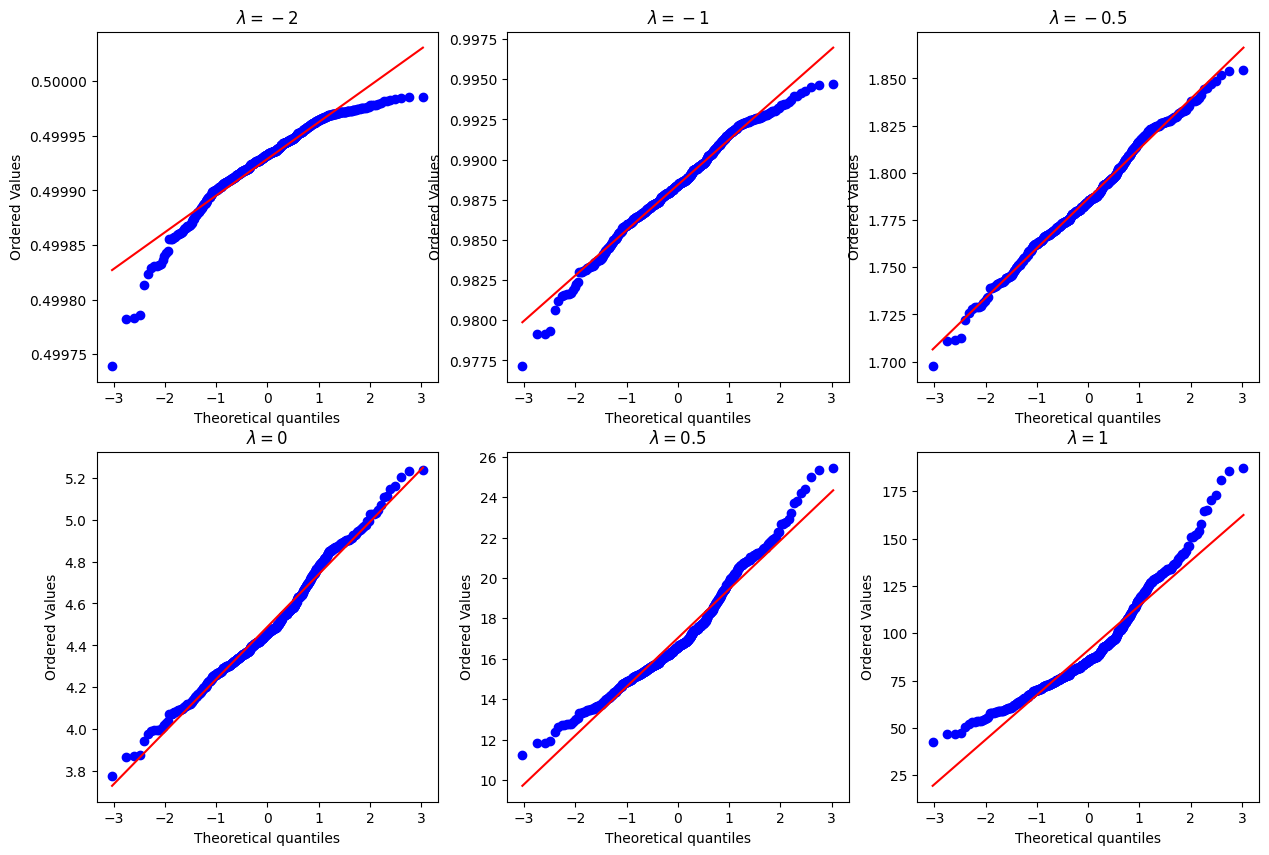
\includegraphics[width=\textwidth]{images/q-q.png}
  \caption{Q-Q plots of various $\lambda$ values}
  \label{fig:q-q}
\end{figure}


\subsection{Calculating Optimal $\lambda$}

We plot multiple $\lambda$ values against the normality of the transformation to calculate the optimal value of $\lambda$.

The normality of the transformation is calculated as Pearson's correlation coefficient between the theoretical quantiles and the observed quantiles.
Pearson's correlation coefficient is calculated as:

\[ r(x, y) = \frac{\overline{xy} - \bar{x} \cdot \bar{y}}{\sigma_x \cdot \sigma_y} \]

\noindent where $x$ and $y$ are two samples, $\bar{x}$ denotes the mean and $\sigma_x$ denotes the standard deviation of $x$.

\autoref{fig:normality} shows the normality for $\lambda \in [-1, 0]$.

\begin{figure}[!ht]
  \centering
  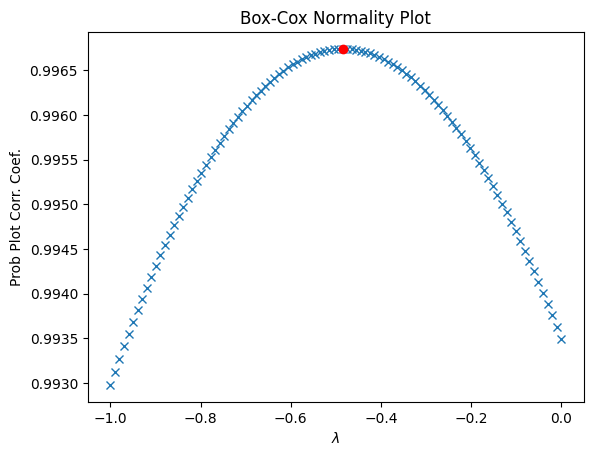
\includegraphics[width=.6\textwidth]{images/normality.png}
  \caption{Box-Cox normality plots of various $\lambda$ values}
  \label{fig:normality}
\end{figure}

\autoref{fig:optimal} shows the histogram of the optimal transformation.

\begin{figure}[!ht]
  \centering
  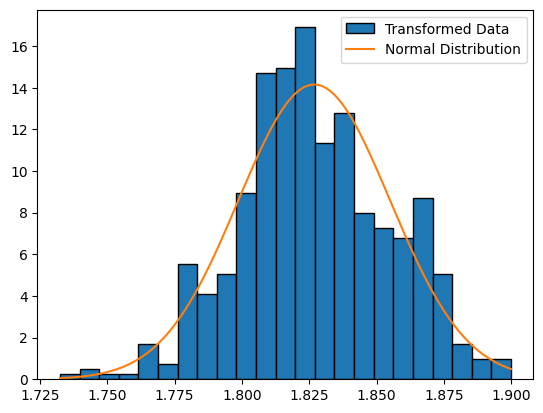
\includegraphics[width=.6\textwidth]{images/optimal-hist.png}
  \caption{Histogram of the optimal transformation of data}
  \label{fig:optimal}
\end{figure}
